% The forecast at test time (Section "Forecast head", "Forecast at test
% time"). The forecaster rolls out r_0, r_1, ... after the encoder latents
% of the context; each r_i is the input of the next step. The head reads
% the whole sequence with a causal mask, and its output at r_i gives the
% quantiles of patch T_p + i. Build: pdflatex test_rollout.tex
\documentclass[tikz,border=1pt]{standalone}
\usepackage[T1]{fontenc}
\usepackage{amsmath}
\usetikzlibrary{arrows.meta,positioning,calc}
\definecolor{clat}{HTML}{A2D6F3}   % encoder latent h: sky blue
\definecolor{cfor}{HTML}{F1CA73}   % rollout forecast r: orange
\begin{document}
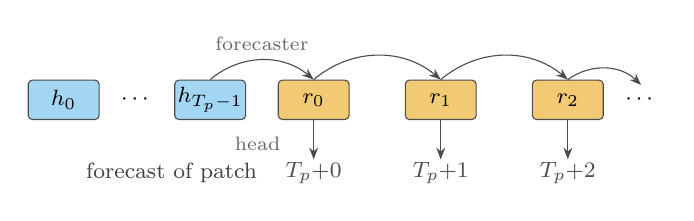
\begin{tikzpicture}[
  font=\footnotesize,
  tok/.style={draw=black!70, rounded corners=1.5pt, minimum width=9mm,
    minimum height=5mm, inner sep=1pt},
  arr/.style={-{Stealth[length=1.5mm]}, black!70},
  node distance=1.5mm,
]
  \node[tok, fill=clat] (h0) {$h_0$};
  \node[right=of h0] (hd) {$\cdots$};
  \node[tok, fill=clat, right=of hd] (hT) {$h_{T_p - 1}$};
  \node[tok, fill=cfor, right=4mm of hT] (r0) {$r_0$};
  \node[tok, fill=cfor, right=7mm of r0] (r1) {$r_1$};
  \node[tok, fill=cfor, right=7mm of r1] (r2) {$r_2$};
  \node[right=of r2] (rd) {$\cdots$};

  % The rollout: the forecaster output at a position is the next input.
  \draw[arr] (hT.north) to[bend left=40] node[above, font=\scriptsize,
    text=black!60] {forecaster} (r0.north);
  \draw[arr] (r0.north) to[bend left=40] (r1.north);
  \draw[arr] (r1.north) to[bend left=40] (r2.north);
  \draw[arr] (r2.north) to[bend left=40] (rd.north);

  % The head: its output at r_i is the forecast of patch T_p + i.
  \foreach \i/\n in {0/r0, 1/r1, 2/r2}
    \draw[arr] (\n.south) -- ++(0, -5mm)
      node[below, inner sep=1pt] (p\i) {$T_p {+} \i$};
  \node[anchor=east, font=\scriptsize, text=black!60]
    at ($(r0.south) + (-3mm, -3mm)$) {head};
  \node[anchor=east, text=black!75] at ($(p0.west) + (-2mm, 0)$)
    {forecast of patch};
\end{tikzpicture}
\end{document}
